\documentclass[slidetop,11pt]{beamer}
%
% Ces deux lignes {\`a} d{\'e}commenter pour sortir 
% le texte en classe article
% \documentclass[class=article,11pt,a4paper]{beamer}
% \usepackage{beamerbasearticle}

% Packages pour les fran\c{c}ais
\usepackage[T1]{fontenc} 
\usepackage[latin1]{inputenc}
%% \usepackage[frenchb]{babel}
% pour un pdf lisible {\`a} l'{\'e}cran si on ne dispose pas 
% des fontes cmsuper ou lmodern
%\usepackage{lmodern}
\usepackage{aeguill}

% Pour afficher le pdf en plein ecran
% (comment{\'e} pour imprimer les transparents et pour les tests)
%\hypersetup{pdfpagemode=FullScreen}

\usetheme{Warsaw}

% Supprimer les icones de navigation (pour les transparents)
\setbeamertemplate{navigation symbols}{}

%------------ fin style beamer -------------------

% Faire appara{\^i}tre un sommaire avant chaque section
% \AtBeginSection[]{
%   \begin{frame}
%   \frametitle{Plan}
%   \medskip
%   %%% affiche en d{\'e}but de chaque section, les noms de sections et
%   %%% noms de sous-sections de la section en cours.
%   \small \tableofcontents[currentsection, hideothersubsections]
%   \end{frame} 
% }

% ----------- Contenu de la page de titre --------
\title{Why how to put TTRPG in your Resume}
\subtitle{To put TableTop Role-Playing Game \newline in a (Professional) Resume and Job Apply} 
%% \subtitle{Cr{\'e}er une Intrigue (cas du JdR)}
\author{Gabriel Chandesris}
% \author{Gabriel Chandesris & Nicolas Dagron}
% \institute{LigueLudique}
% \institute{\includegraphics[width=5cm]{img/ligueludique-1.png}}
% \institute{\includegraphics[width=5cm]{img/ligueludique-1.png}~\includegraphics[width=5cm]{img/logo-studio-infinite-2.png}}
\date{\today} %% \date{03 Janvier 2018} %% \date{\today} %% \date{03 Janvier 2018}
%% \logo{
\includegraphics[height=0.5cm]{img/logo_glider.png}}

% ----------- Nom des diff{\'e}rentes parties --------

%% Mis au fur et {\`a} mesure...

% ------------------------------------------------
% -------------   D{\'e}but document   ---------------
% ------------------------------------------------
\begin{document}
%--------- {\'e}criture de la page de titre ----------
% avec la commande frame simplifi{\'e}e
\frame[plain]{\titlepage}
%

%------------------ Sommaire ---------------

\begin{frame}
	\frametitle{Table Of Content}
	\small \tableofcontents[hideallsubsections]
\end{frame} 

\def\sectionItitle{Base Content}
\section{ \sectionItitle }
\begin{frame}
	\frametitle{ \sectionItitle }
	\tableofcontents[sections=1,currentsection,subsectionstyle=show/shaded/hide]
\end{frame} 

\def\subsectionTtitle{Image}

\subsection{ \subsectionTtitle~(1)  -- Game Night }
\begin{frame}
	\frametitle{ \subsectionTtitle~(1) -- Game Night }
	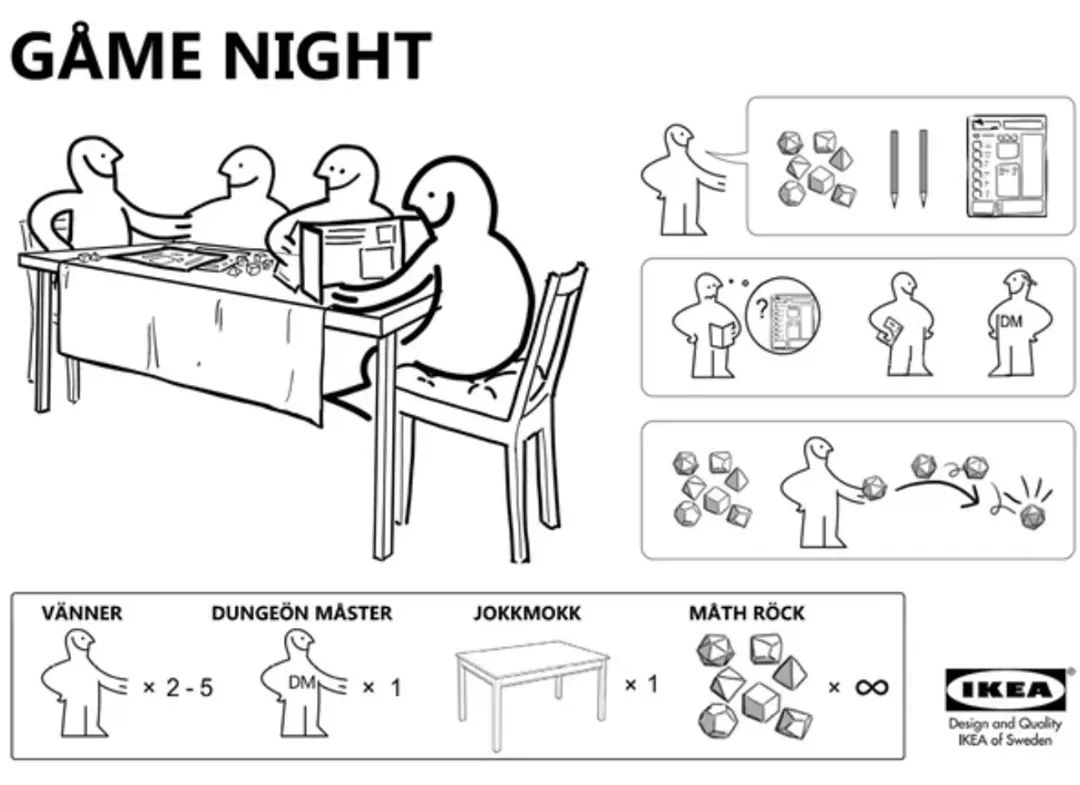
\includegraphics[width=0.95\textwidth]{132926019-440f4a99-81b7-45ea-8c4a-92993496556c.jpg} 
\end{frame} 

\subsection{ \subsectionTtitle~(2)  -- How to include ... (1)}
\begin{frame}
	\frametitle{ \subsectionTtitle~(2) -- How to include ... (1)}
	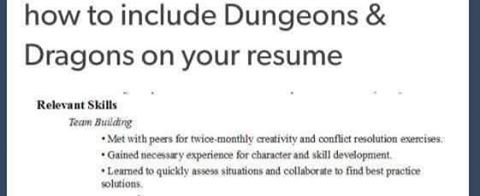
\includegraphics[width=0.95\textwidth]{132926053-04fe2306-b5bd-4dc2-8403-439809517410.jpg} 
\end{frame} 

\subsection{ \subsectionTtitle~(3) -- How to include ... (2)}
\begin{frame}
	\frametitle{ \subsectionTtitle~(3) -- How to include ... (2)}
	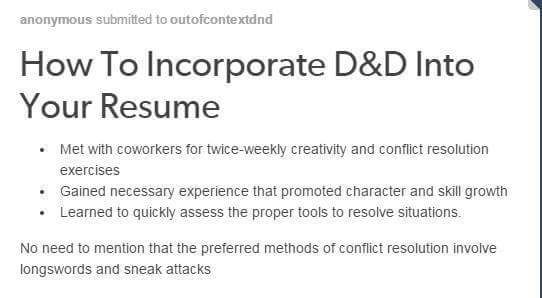
\includegraphics[width=0.95\textwidth]{132926092-476f735d-d1cc-4ee4-9460-3e468ff5cd7a.jpeg} 
\end{frame}

\subsection{ \subsectionTtitle~(4) -- How to include ... (3)}
\begin{frame}
	\frametitle{ \subsectionTtitle~(4) -- How to include ... (3)}
	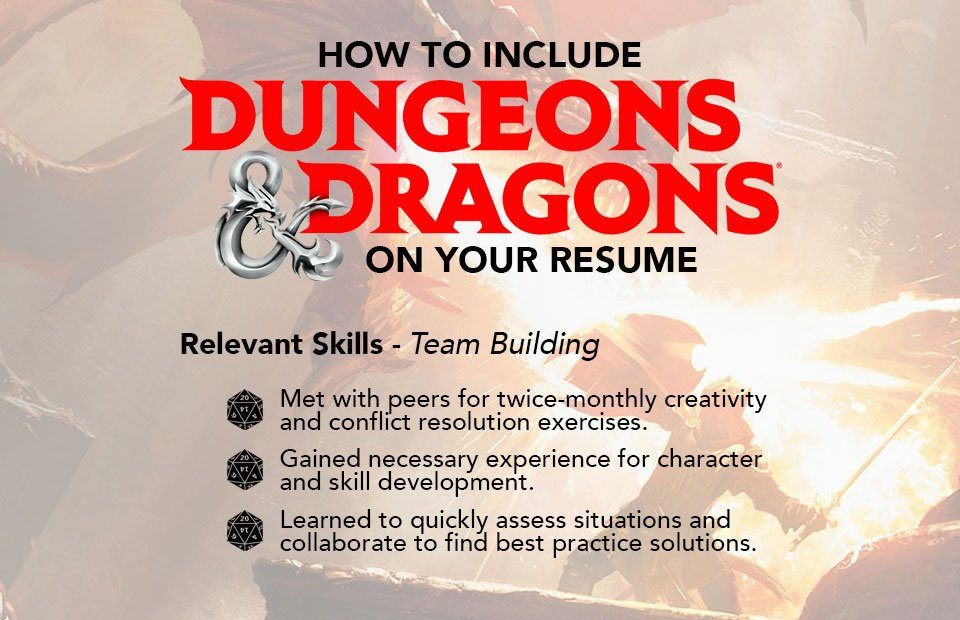
\includegraphics[width=0.95\textwidth]{132926163-fc6cf9bd-b35c-49b3-9366-3df360482e7c.jpg} 
\end{frame}

\subsection{ \subsectionTtitle~(5) -- What We Do ... An example of routine. }
\begin{frame}
	\frametitle{ \subsectionTtitle~(5) -- What We Do ... An example of routine. }
	\begin{center} 
		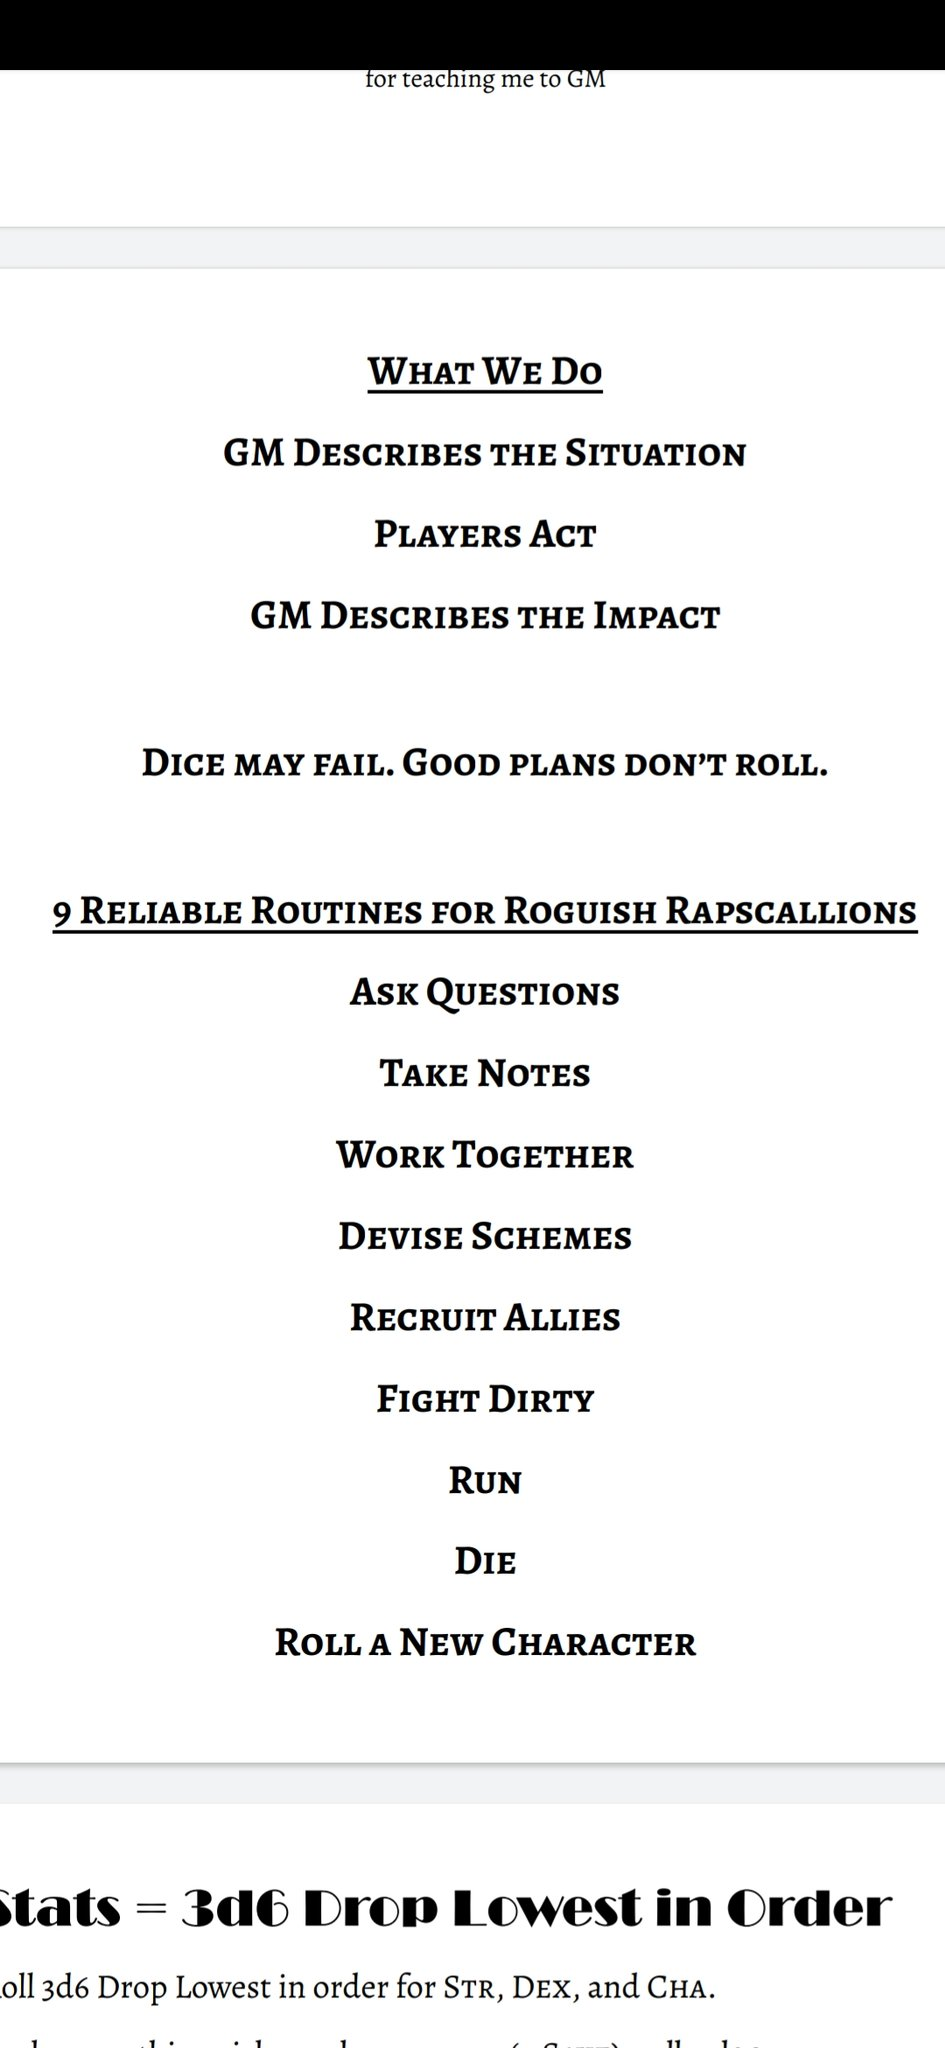
\includegraphics[height=0.95\textheight]{132926147-ad61d89d-4f36-48c8-acac-54cecfe960db.jpeg}
	\end{center} 
\end{frame}

\def\sectionIItitle{Basics}
\section{ \sectionIItitle }
\begin{frame}
	\frametitle{ \sectionIItitle }
	\tableofcontents[sections=2,currentsection,subsectionstyle=show/shaded/hide]
\end{frame} 

\subsection{ Skills }
\begin{frame}
	\frametitle{ Some indicated basics which apply ... }
	\begin{itemize}
		\item Meet coworkers / peers regularly ; 
		\item Conflict resolutions exercices ;  
		\item Gain necessary experience ; 
		\item Skill developments ; 
		\item Learned to quick asset situations ; 
		\item Collaborate to find best practice solutions ; 
		\item Team Building ; 
	\end{itemize}
\end{frame}

\subsection{ Others (?) }
\begin{frame}
	\frametitle{ More than the basics ... }
	\begin{itemize}
		\item World Building ; 
		\item Organize / co-organize meetings ; 
		\item Planification and resources ; 
		\item Optimisation of available resources ; 
		\item Preparation of sessions ; 
	\end{itemize}
\end{frame}

\subsection{ More than "Game" }
\begin{frame}
	\frametitle{ Social encounters ... }
	\begin{itemize}
		\item Is it only "gaming" or more than that ?
		\item ... 
	\end{itemize}
\end{frame}

\def\sectionIIItitle{What's next in redaction}
\section{ \sectionIIItitle }
\begin{frame}
	\frametitle{ \sectionIIItitle }
	\tableofcontents[sections=3,currentsection,subsectionstyle=show/shaded/hide]
\end{frame} 

\subsection{ Skills }
\begin{frame}
	\frametitle{ Skills ... }
	\begin{itemize}
		\item ... 
		\item ... 
		\item ... 
	\end{itemize}
\end{frame}

\subsection{ Behaviours }
\begin{frame}
	\frametitle{ Behaviours ... }
	\begin{itemize}
		\item ... 
		\item ... 
		\item ... 
	\end{itemize}
\end{frame}

\subsection{ Expectations }
\begin{frame}
	\frametitle{ Expectations ... }
	\begin{itemize}
		\item ... 
		\item ... 
		\item ... 
	\end{itemize}
\end{frame}

\end{document}
